% -*- TeX -*- -*- UK -*- -*- Soft -*-

\chapter{Introduction to Markov Chains}
\label{chap:IntroductiontoMarkovChains}

This chapter is a verbatim copy of a blog \cite{JosephRoccaMarkovChains2019} by Joseph Rocca.


\textit{Definitions, properties and PageRank example.}

\section{Introduction}

In 1998, Lawrence Page, Sergey Brin, Rajeev Motwani and Terry Winograd published "The PageRank Citation Ranking: Bringing Order to the Web", an article in which they introduced the now famous PageRank algorithm at the origin of Google. A little bit more than two decades later, Google has became a giant and, even if the algorithm has evolved a lot, the PageRank is still a "symbol" of the Google ranking algorithm (even if few people can really say the weight it still occupies in the algorithm).

From a theoretical point of view, it is interesting to notice that one common interpretation of the PageRank algorithm relies on the simple but fundamental mathematical notion of Markov chains. We will see in this article that Markov chains are powerful tools for stochastic modelling that can be useful to any data scientist. More especially, we will answer basic questions such as: what are Markov chains, what good properties do they have and what can be done with them?

\section{Outline}
In the first section we will give the basic definitions required to understand what Markov chains are. In the second section, we will discuss the special case of finite state space Markov chains. Then, in the third section we will discuss some elementary properties of Markov chains and will illustrate these properties with many little examples. Finally, in the fourth section we will make the link with the PageRank algorithm and see on a toy example how Markov chains can be used for ranking nodes of a graph.

Note. Basics of probability and linear algebra are required in this post. In particular, the following notions will be used: 
\href{https://en.wikipedia.org/wiki/Conditional_probability}{conditional probability}, 
\href{https://en.wikipedia.org/wiki/Eigenvalues_and_eigenvectors}{eigenvector}, and 
\href{https://en.wikipedia.org/wiki/Law_of_total_probability}{law of total probability}.

\section{What are Markov chains?}
\subsection{Random variables and random processes}

Before introducing Markov chains, let's start with a quick reminder of some basic but important notions of probability theory.

First, in non-mathematical terms, a \textbf{random variable} $X$ is a variable whose value is defined as the outcome of a random phenomenon. This outcome can be a number (or "number-like", including vectors) or not. For example we can define a random variable as the outcome of rolling a dice (number) as well as the output of flipping a coin (not a number, unless you assign, for example, 0 to head and 1 to tail). Notice also that the space of possible outcomes of a random variable can be discrete or continuous: for example, a normal random variable is continuous whereas a poisson random variable is discrete.

We can then define a \textbf{random process} (also called stochastic process) as a collection of random variables indexed by a set $T$ that often represent different instants of time (we will assume that in the following). The two most common cases are: either $T$ is the set of natural numbers (discrete time random process) or $T$ is the set of real numbers (continuous time random process). For example, flipping a coin every day defines a discrete time random process whereas the price of a stock market option varying continuously defines a continuous time random process. The random variables at different instant of time can be independent to each other (coin flipping example) or dependent in some way (stock price example) as well as they can have continuous or discrete state space (space of possible outcomes at each instant of time), see Figure~\ref{fig:p05c07-snip01}.

\begin{figure*}[h]
    \centering
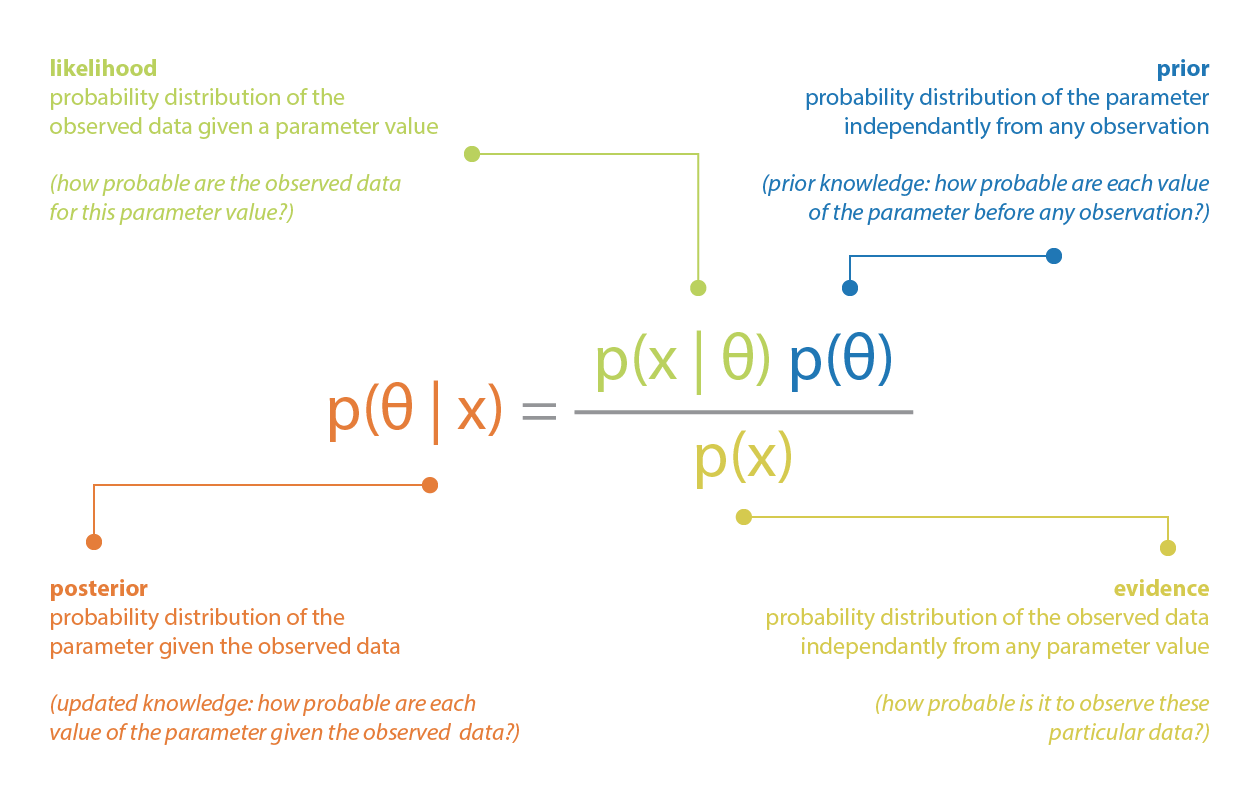
\includegraphics[width=\textwidth]{pic/p05c07-snip01.png}
    \caption{Different kind of random processes (discrete/continuous in space/time)}
    \label{fig:p05c07-snip01}
\end{figure*}


\subsection{Markov property and Markov chain}

There exists some well known families of random processes: gaussian processes, poisson processes, autoregressive models, moving-average models, Markov chains and others. These particular cases have, each, specific properties that allow us to better study and understand them.

One property that makes the study of a random process much easier is the "Markov property". In a very informal way, the Markov property says, for a random process, that if we know the value taken by the process at a given time, we won't get any additional information about the future behaviour of the process by gathering more knowledge about the past. Stated in slightly more mathematical terms, for any given time, the conditional distribution of future states of the process given present and past states depends only on the present state and not at all on the past states (\textbf{memoryless property}). A random process with the Markov property is called \textbf{Markov process}.



\begin{figure}[h]
    \centering
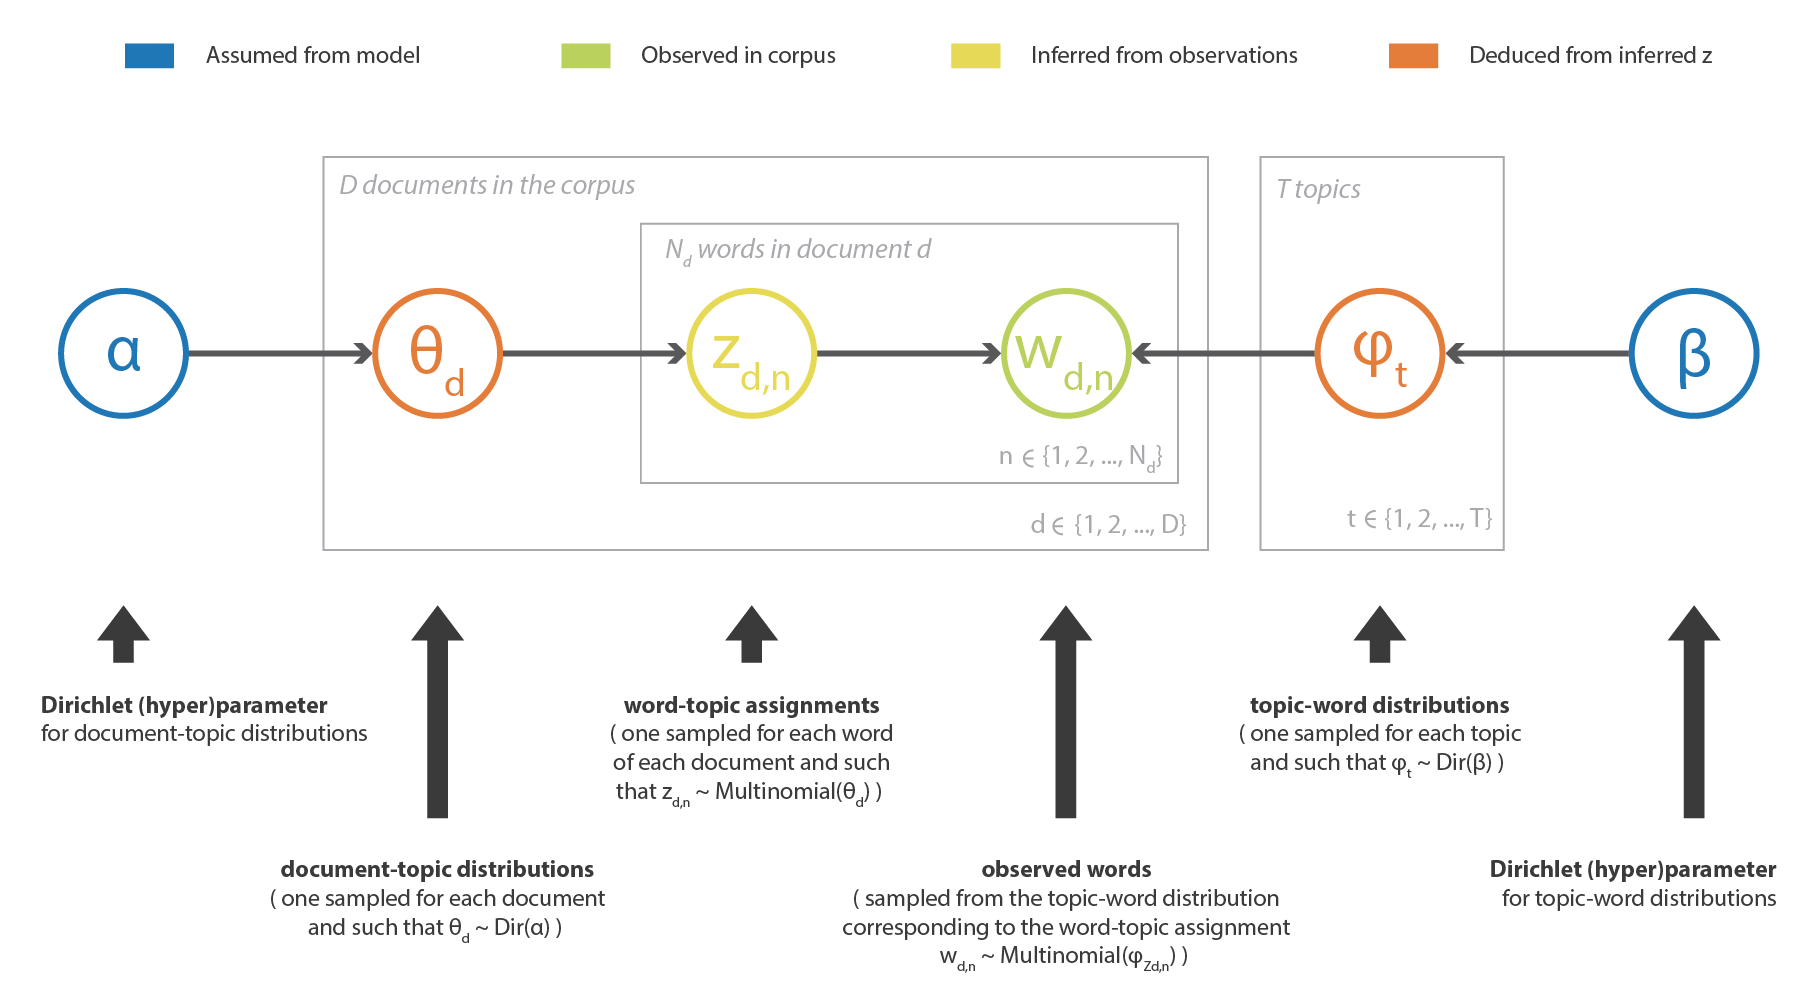
\includegraphics[width=\textwidth]{pic/p05c07-snip02.png}
    \caption[The Markov does not learn about the future by gathering information about the past]{The Markov property expresses the fact that at a given time step and knowing the current state, we won't get any additional information about the future by gathering information about the past}
    \label{fig:p05c07-snip02}
\end{figure}




Based on the previous definition, we can now define "homogenous discrete time Markov chains" (that will be denoted "Markov chains" for simplicity in the following). A \textbf{Markov chain} is a Markov process with discrete time and discrete state space. So, a Markov chain is a discrete sequence of states, each drawn from a discrete state space (finite or not), and that follows the Markov property.

Mathematically, we can denote a Markov chain by
\begin{equation}X=\left(X_{n}\right)_{n \in \mathrm{N}}=\left(X_{0}, X_{1}, X_{2}, \ldots\right)\end{equation}
where at each instant of time the process takes its values in a discrete set $E$ such that
\begin{equation}X_{n} \in E \quad \forall n \in \mathbb{N}\end{equation}
Then, the Markov property implies that we have
\begin{equation}
\mathbb{P}\left(X_{n+1}=s_{n+1} | X_{n}=s_{n}, X_{n-1}=s_{n-1}, X_{n-2}=s_{n-2}, \ldots\right)=\mathbb{P}\left(X_{n+1}=s_{n+1} | X_{n}=s_{n}\right)
\end{equation}

Notice once again that this last formula expresses the fact that for a given historic (where I am now and where I was before), the probability distribution for the next state (where I go next) only depends on the current state and not on the past states.

Note. We have decided to describe only basic homogenous discrete time Markov chains in this introductory post. However, there also exists inhomogenous (time dependent) and/or time continuous Markov chains. We won't discuss these variants of the model in the following. Notice also that the definition of the Markov property given above is extremely simplified: the true mathematical definition involves the notion of filtration that is far beyond the scope of this modest introduction.

\subsection{Characterising the random dynamic of a Markov chain}

We have introduced in the previous subsection a general framework matched by any Markov chain. Let's now see what we do need in order to define a specific "instance" of such a random process.

Notice first that the full characterisation of a discrete time random process that doesn't verify the Markov property can be painful: the probability distribution at a given time can depend on one or multiple instants of time in the past and/or the future. All these possible time dependences make any proper description of the process potentially difficult.

However, thanks to the Markov property, the dynamic of a Markov chain is pretty easy to define. Indeed, we only need to specify two things: an \textbf{initial probability distribution} (that is a probability distribution for the instant of time $n=0$) denoted
\begin{equation}\mathbb{P}\left(X_{0}=s\right)=q_{0}(s) \quad \forall s \in E\end{equation}
and a \textbf{transition probability kernel} (that gives the probabilities that a state, at time $n+1$, succeeds to another, at time n, for any pair of states) denoted
\begin{equation}\mathbb{P}\left(X_{n+1}=s_{n+1} | X_{n}=s_{n}\right)=p\left(s_{n}, s_{n+1}\right) \quad \forall\left(s_{n+1}, s_{n}\right) \in E \times E\end{equation}
With the previous two objects known, the full (probabilistic) dynamic of the process is well defined. Indeed, the probability of any realisation of the process can then be computed in a recurrent way.

Assume for example that we want to know the probability for the first 3 states of the process to be $(s0, s1, s2)$. So, we want to compute the probability
\begin{equation}\mathbb{P}\left(X_{0}=s_{0}, X_{1}=s_{1}, X_{2}=s_{2}\right)\end{equation}
Here, we use the law of total probability stating that the probability of having $(s0, s1, s2)$ is equal to the probability of having first $s0$, multiplied by the probability of having $s1$ given we had $s0$ before, multiplied by the probability of having finally $s2$ given that we had, in order, $s0$ and $s1$ before. Mathematically, it can be written
\begin{equation}\mathbb{P}\left(X_{0}=s_{0}, X_{1}=s_{1}, X_{2}=s_{2}\right)=\mathbb{P}\left(X_{0}=s_{0}\right) \mathbb{P}\left(X_{1}=s_{1} | X_{0}=s_{0}\right) \mathbb{P}\left(X_{2}=s_{2} | X_{0}=s_{0}, X_{1}=s_{1}\right)\end{equation}
Then appears the simplification given by the Markov assumption. Indeed, for long chains we would obtain for the last states heavily conditional probabilities. However, in a Markov case we can simplify this expression using that
\begin{equation}\mathbb{P}\left(X_{2}=s_{2} | X_{0}=s_{0}, X_{1}=s_{1}\right)=\mathbb{P}\left(X_{2}=s_{2} | X_{1}=s_{1}\right)\end{equation}
such that we have
\begin{equation}\begin{aligned}
\mathbb{P}\left(X_{0}=s_{0}, X_{1}=s_{1}, X_{2}=s_{2}\right) &=\mathbb{P}\left(X_{0}=s_{0}\right) \mathbb{P}\left(X_{1}=s_{1} | X_{0}=s_{0}\right) \mathbb{P}\left(X_{2}=s_{2} | X_{1}=s_{1}\right) \\
&=q_{0}\left(s_{0}\right) p\left(s_{0}, s_{1}\right) p\left(s_{1}, s_{2}\right)
\end{aligned}\end{equation}
As they fully characterise the probabilistic dynamic of the process, many other more complex events can then be computed only based on both the initial probability distribution $q0$ and the transition probability kernel $p$. One last basic relation that deserves to be given is the expression of the probability distribution at time $n+1$ expressed relatively to the probability distribution at time $n$
\begin{equation}q_{n+1}\left(s_{n+1}\right) \stackrel{\text { def }}{=} \mathbb{P}\left(X_{n+1}=s_{n+1}\right)=\sum_{s \in E} \mathbb{P}\left(X_{n}=s\right) \mathbb{P}\left(X_{n+1}=s_{n+1} | X_{n}=s\right)=\sum_{s \in E} q_{n}(s) p\left(s, s_{n+1}\right)\end{equation}

\section{Finite state space Markov chains}
\subsection{Matrix and graph representation}

We assume here that we have a finite number $N$ of possible states in $E$:
\begin{equation}E=\left\{e_{1}, e_{2}, \dots, e_{N}\right\}\end{equation}
Then, the initial probability distribution can be described by a \textbf{row vector} $q0$ of size $N$ and the transition probabilities can be described by a matrix $p$ of size $N$ by $N$ such that

$\left(q_{0}\right)_{i}=q_{0}\left(e_{i}\right)=\mathbb{P}\left(X_{0}=e_{i}\right)$\\
$p_{i, j}=p\left(e_{i}, e_{j}\right)=\mathbb{P}\left(X_{n+1}=e_{j} | X_{n}=e_{i}\right)$
(independent of n)

The advantage of such notation is that if we note denote the probability distribution at step $n$ by a raw vector $q_n$ such that its components are given by
\begin{equation}
\left(q_{n}\right)_{i}=q_{n}\left(e_{i}\right)=\mathbb{P}\left(X_{n}=e_{i}\right)
\end{equation}
then the simple matrix relations thereafter hold
\begin{equation}
q_{n+1}=q_{n} p \quad q_{n+2}=q_{n+1} p=\left(q_{n} p\right) p=q_{n} p^{2} \quad \ldots \quad q_{n+m}=q_{n} p^{m}
\end{equation}
(the proof won't be detailed here but can be recovered very easily).

\begin{figure*}[h]
    \centering
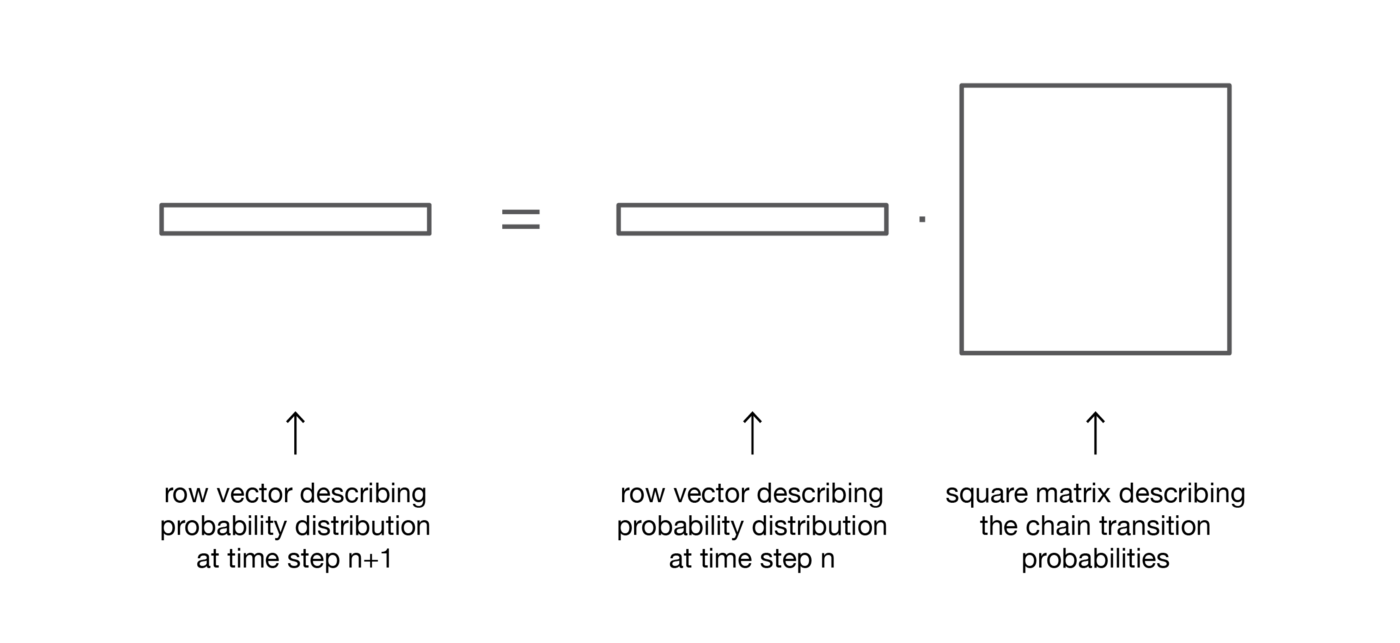
\includegraphics[width=\textwidth]{pic/p05c07-snip03.png}
    \caption[Obtain the probability distribution for the next time step]{When right multiplying a row vector representing probability distribution at a given time step by the transition probability matrix, we obtain the probability distribution at the next time step}
    \label{fig:p05c07-snip03}
\end{figure*}

So, we see here that evolving the probability distribution from a given step to the following one is as easy as right multiplying the row probability vector of the initial step by the matrix $p$. This also implies that we have

$p_{i, j}=\mathbb{P}\left(X_{n+1}=e_{j} | X_{n}=e_{i}\right) \equiv$ probability of going from $e_{i}$ to $e_{j}$ in 1 step \\
$\left(p^{2}\right)_{i, j}=\mathbb{P}\left(X_{n+2}=e_{j} | X_{n}=e_{i}\right) \equiv$ probability of going from $e_{i}$ to $e_{j}$ in 2 steps\\
$\left(p^{m}\right)_{i, j}=\mathbb{P}\left(X_{n+m}=e_{j} | X_{n}=e_{i}\right) \equiv$ probability of going from $e_{i}$ to $e_{j}$ in $\mathrm{m}$ steps

The random dynamic of a finite state space Markov chain can easily be represented as a valuated oriented graph such that each node in the graph is a state and, for all pairs of states $(e_i, e_j)$, there exists an edge going from $e_i$ to $e_j$ if $p(e_i,e_j)>0$. The value of the edge is then this same probability $p(e_i,e_j)$.

\subsection{Example: the Towards Data Science reader}

Let's take a simple example to illustrate all this. Consider the daily behaviour of a fictive Towards Data Science reader. For each day, there are 3 possible states: the reader doesn't visit TDS this day ($N$), the reader visits TDS but doesn't read a full post ($V$) and the reader visits TDS and read at least one full post ($R$). So, we have the following state space
\begin{equation}E=\{N, V, R\}\end{equation}
Assume that at the first day this reader has 50\% chance to only visit TDS and 50\% chance to visit TDS and read at least one article. The vector describing the initial probability distribution ($n=0$) is then
\begin{equation}q_{0}=(0.0,0.5,0.5)\end{equation}
Imagine also that the following probabilities have been observed:
\begin{enumerate}
\item when the reader doesn't visit TDS a day, he has 25\% chance of still not visiting the next day, 50\% chance to only visit and 25\% to visit and read

\item when the reader visits TDS without reading a day, he has 50\% chance to visit again without reading the next day and 50\% to visit and read

\item when the reader visits and read a day, he has 33\% chance of not visiting the next day (\textit{hope that this post won't have this kind of effect!}), 33\% chance to only visit and 34\% to visit and read again
\end{enumerate}


Then, we have the following transition matrix
\begin{equation}p=\left(\begin{array}{lll}
0.25 & 0.50 & 0.25 \\
0.00 & 0.50 & 0.50 \\
0.33 & 0.33 & 0.34
\end{array}\right)\end{equation}
Based on the previous subsection, we know how to compute, for this reader, the probability of each state for the second day ($n=1$)
\begin{equation}q_{1}=q_{0} p=(0.0,0.5,0.5)\left(\begin{array}{ccc}
0.25 & 0.50 & 0.25 \\
0.00 & 0.50 & 0.50 \\
0.33 & 0.33 & 0.34
\end{array}\right)=(0.165,0.415,0.420)\end{equation}
Finally, the probabilistic dynamic of this Markov chain can be graphically represented as follows

\begin{figure*}[h]
    \centering
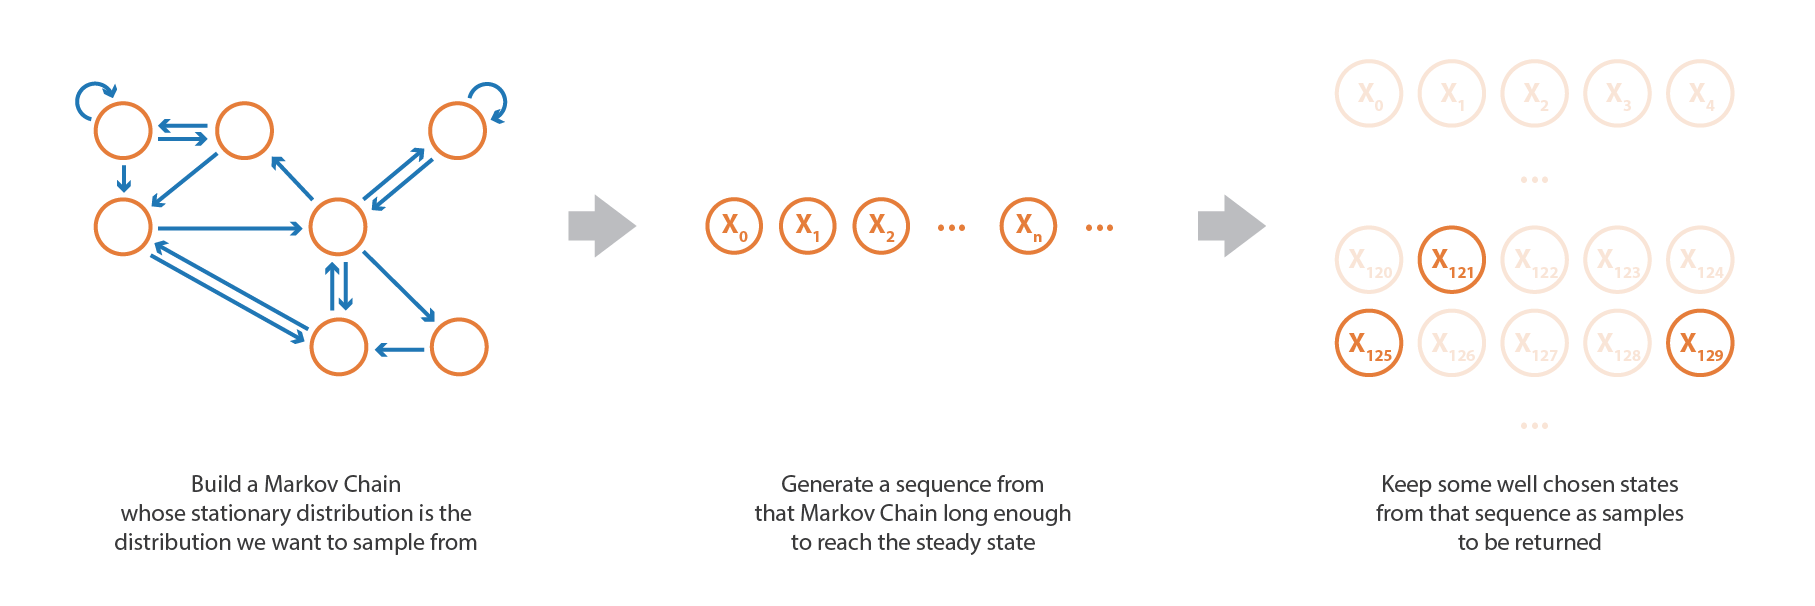
\includegraphics[width=\textwidth]{pic/p05c07-snip04.png}
    \caption{Graph representation of the Markov chain modelling our fictive TDS reader behaviour}
    \label{fig:p05c07-snip04}
\end{figure*}

.

\section{Markov Chains properties}

In this section, we will only give some basic Markov chains properties or characterisations. The idea is not to go deeply into mathematical details but more to give an overview of what are the points of interest that need to be studied when using Markov chains. As we have seen that in the finite state space case we can picture a Markov chain as a graph, notice that we will use graphical representation to illustrate some of the properties bellow. However, one should keep in mind that these properties are not necessarily limited to the finite state space case.

\subsection{Reducibility, periodicity, transience and recurrence}
Let's start, in this subsection, with some classical ways to characterise a state or an entire Markov chain.

First, we say that a Markov chain is \textbf{irreducible} if it is possible to reach any state from any other state (not necessarily in a single time step). If the state space is finite and the chain can be represented by a graph, then we can say that the graph of an irreducible Markov chain is strongly connected (graph theory).

\begin{figure*}[h]
    \centering
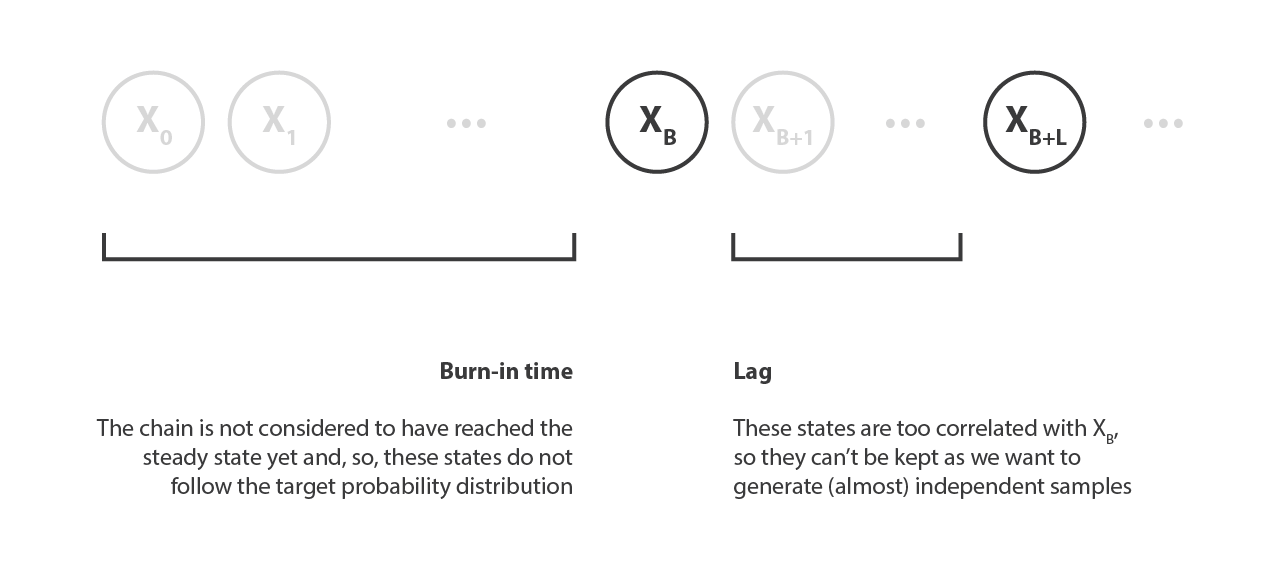
\includegraphics[width=\textwidth]{pic/p05c07-snip05.png}
    \caption[Illustration of the irreducibility property]{Illustration of the irreducibility property. The chain on the left is not irreducible: from 3 or 4 we can't reach 1 or 2. The chain on the right (one edge has been added) is irreducible: each state can be reached from any other state}
    \label{fig:p05c07-snip05}
\end{figure*}


A state has period $k$ if, when leaving it, any return to that state requires a multiple of $k$ time steps ($k$ is the greatest common divisor of all the possible return path length). If $k = 1$, then the state is said to be aperiodic and a whole Markov chain is \textbf{aperiodic} if all its states are aperiodic. For an irreducible Markov chain, we can also mention the fact that if one state is aperiodic then all states are aperiodic.



\begin{figure*}[h]
    \centering
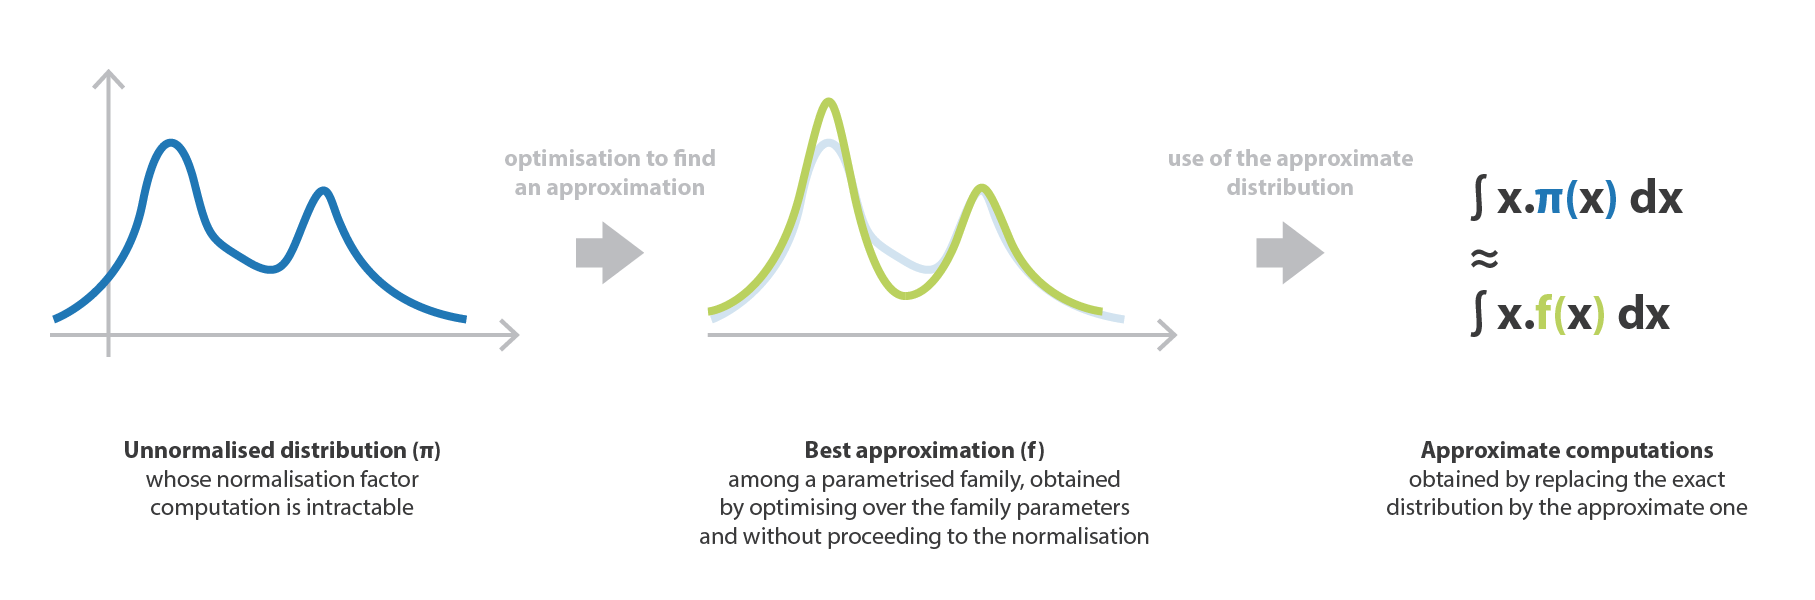
\includegraphics[width=\textwidth]{pic/p05c07-snip06.png}
    \caption[Illustration of the periodicity property]{Illustration of the periodicity property. The chain on the left is 2-periodic: when leaving any state, it always takes a multiple of 2 steps to come back to it. The chain on the right is 3-periodic}
    \label{fig:p05c07-snip06}
\end{figure*}

A state is \textbf{transient} if, when we leave this state, there is a non-zero probability that we will never return to it. Conversely, a state is \textbf{recurrent} if we know that we will return to that state, in the future, with probability 1 after leaving it (if it is not transient).



\begin{figure*}[h]
    \centering
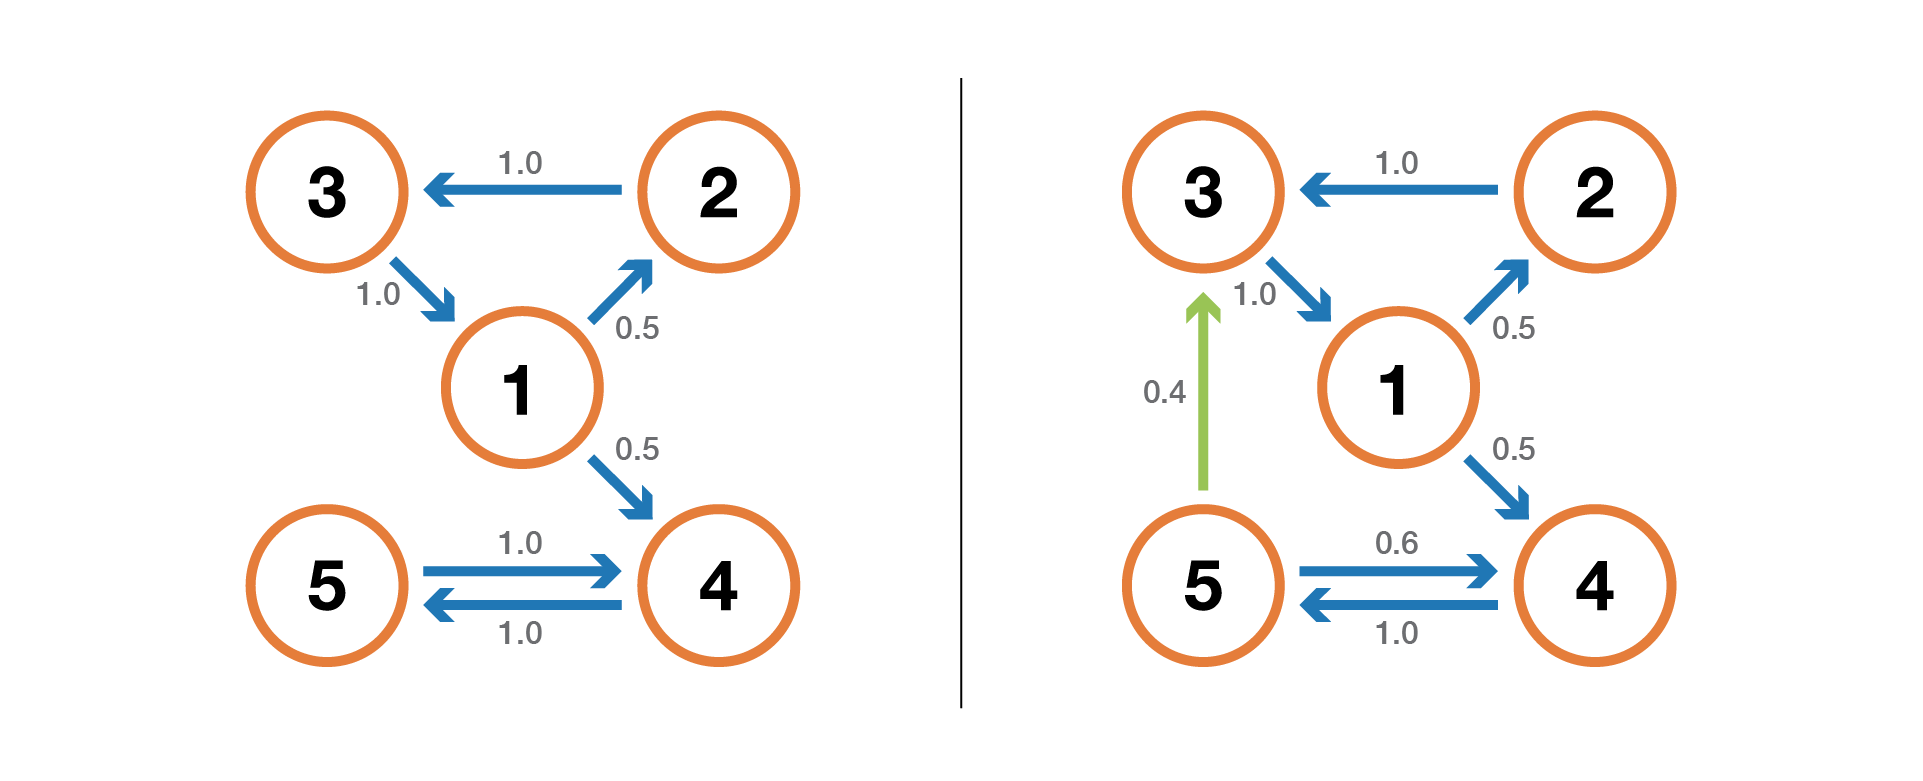
\includegraphics[width=\textwidth]{pic/p05c07-snip07.png}
    \caption[Illustration of the recurrence/transience property.]{Illustration of the recurrence/transience property. The chain of the left is such that: 1, 2 and 3 are transient (when leaving these points we can't be absolutely sure that we will come back to them) and 3-periodic whereas 4 and 5 are recurrent (when leaving these points we are absolutely sure that we will come back to them at some time) and 2-periodic. The chain on the right has one more edge that makes the full chain recurrent and aperiodic}
    \label{fig:p05c07-snip07}
\end{figure*}

For a recurrent state, we can compute the mean recurrence time that is the \textbf{expected return time} when leaving the state. Notice that even if the probability of return is equal to 1, it doesn't mean that the expected return time is finite. So, among the recurrent states, we can make a difference between \textbf{positive recurrent} state (finite expected return time) and \textbf{null recurrent } state (infinite expected return time).

\subsection{Stationary distribution, limiting behaviour and ergodicity}

We discuss, in this subsection, properties that characterise some aspects of the (random) dynamic described by a Markov chain.

A probability distribution $\pi$ over the state space $E$ is said to be a \textbf{stationary distribution} if it verifies
\begin{equation}\pi\left(e^{\prime}\right)=\sum_{e \in E} \pi(e) p\left(e, e^{\prime}\right) \quad \forall e^{\prime} \in E\end{equation}
As we have\\
\begin{tabular}{rcl}
$\pi\left(e^{\prime}\right)$&$=$& probability of being in $e^{\prime}$ at the current step \\
$\sum_{e \in E} \pi(e) p\left(e, e^{\prime}\right)$&$=$& probability of being in $e^{\prime}$ at the next step
\end{tabular}

Then a stationary distribution verifies

probability of being in $e^{\prime}$ at the current step
 $=$ probability of being in $e^{\prime}$ at the next step

By definition, a stationary probability distribution is then such that it doesn't evolve through the time. So if the initial distribution $q$ is a stationary distribution then it will stay the same for all future time steps. If the state space is finite, $p$ can be represented by a matrix and $\pi$ by a raw vector and we then have
\begin{equation}\pi=\pi p=\pi p^{2}=\dots\end{equation}
Once more, it expresses the fact that a stationary probability distribution doesn't evolve through the time (as we saw that right multiplying a probability distribution by $p$ allows to compute the probability distribution at the next time step). Notice that an irreducible Markov chain has a stationary probability distribution if and only if all of its states are positive recurrent.

Another interesting property related to stationary probability distribution is the following. If the chain is recurrent positive (so that there exists a stationary distribution) and aperiodic then, no matter what the initial probabilities are, the probability distribution of the chain converges when time steps goes to infinity: the chain is said to have a \textbf{limiting distribution} that is nothing else than the stationary distribution. In the general case it can be written
\begin{equation}\lim _{n \rightarrow \infty} \mathbb{P}\left(X_{n}=e^{\prime} | X_{0}=e\right)=\lim _{n \rightarrow \infty} p^{n}\left(e, e^{\prime}\right)=\pi\left(e^{\prime}\right) \quad \forall\left(e, e^{\prime}\right) \in E \times E\end{equation}
Let's emphasise once more the fact that there is no assumption on the initiale probability distribution: the probability distribution of the chain converges to the stationary distribution (equilibrium distribution of the chain) regardless of the initial setting.

Finally, \textbf{ergodicity} is another interesting property related to the behaviour of a Markov chain. If a Markov chain is irreducible then we also say that this chain is "ergodic" as it verifies the following ergodic theorem. Assume that we have an application $f(.)$ that goes from the state space $E$ to the real line (it can be, for example, the cost to be in each state). We can define the mean value that takes this application along a given trajectory (temporal mean). For the $n$-th first terms it is denoted by
\begin{equation}\frac{1}{n}\left(f\left(X_{0}\right)+f\left(X_{1}\right)+\ldots+f\left(X_{n-1}\right)\right)=\frac{1}{n} \sum_{i=0}^{n-1} f\left(X_{i}\right)\end{equation}
We can also compute the mean value of application f over the set $E$ weighted by the stationary distribution (spatial mean) that is denoted by
\begin{equation}\sum_{e \in E} \pi(e) f(e)\end{equation}
Then ergodic theorem tells us that the temporal mean when trajectory become infinitely long is equal to the spatial mean (weighted by stationary distribution). The ergodic property can be written
\begin{equation}\lim _{n \rightarrow \infty} \frac{1}{n} \sum_{i=0}^{n-1} f\left(X_{i}\right)=\sum_{e \in E} \pi(e) f(e)\end{equation}
Stated in another way, it says that, at the limit, the early behaviour of the trajectory becomes negligible and only the long run stationary behaviour really matter when computing the temporal mean.

\subsection{Back to our TDS reader example}

We consider our TDS reader example again. In this simple example, the chain is clearly irreducible, aperiodic and all the states are recurrent positive.

In order to show the kind of interesting results that can be computed with Markov chains, we want to look at the mean recurrence time for the state $R$ (state "visit and read"). In other words, we would like to answer the following question: when our TDS reader visits and reads a given day, how many days do we have to wait in average before he visits and reads again? Let's try to get an intuition of how to compute this value.

First, we denote

$m\left(e, e^{\prime}\right) \equiv$ mean time to go from state $e$ to state $e^{\prime}$

So we want to compute here $m(R,R)$. Reasoning on the first step reached after leaving $R$, we get

\begin{equation}\begin{aligned}
m(R, R) &=p_{R, N}(1+m(N, R))+p_{R, V}(1+m(V, R))+p_{R, R}(1+0) \\
&=1+\left[m(N, R) \times p_{R, N}+m(V, R) \times p_{R, V}+0 \times p_{R, R}\right] \\
&=1+m(N, R) \times p_{R, N}+m(V, R) \times p_{R, V}
\end{aligned}\end{equation}

This expression, however, requires to know $m(N,R)$ and $m(V,R)$ to compute $m(R,R)$. These two quantities can be expressed the same way
\begin{equation}\begin{aligned}
m(N, R) &=1+m(N, R) \times p_{N, N}+m(V, R) \times p_{N, V} \\
m(V, R) &=1+m(N, R) \times p_{V, N}+m(V, R) \times p_{V, V}
\end{aligned}\end{equation}
So, we have 3 equations with 3 unknowns and, when we solve this system, we obtain $m(N,R)$ = 2.67, $m(V,R)$ = 2.00 and $m(R,R)$ = 2.54. The value of the mean recurrence time of state $R$ is then 2.54. So, we see that, with a few linear algebra, we managed to compute the mean recurrence time for the state $R$ (as well as the mean time to go from $N$ to $R$ and the mean time to go from $V$ to $R$).

To conclude this example, let's see what the stationary distribution of this Markov chain is. To determine the stationary distribution, we have to solve the following linear algebra equation
\begin{equation}\pi=\pi p \Longleftrightarrow\left(\pi_{N} \quad \pi_{V} \quad \pi_{R}\right)=\left(\begin{array}{ccc}
\pi_{N} & \pi_{V} & \pi_{R}
\end{array}\right)\left(\begin{array}{ccc}
0.25 & 0.50 & 0.25 \\
0.00 & 0.50 & 0.50 \\
0.33 & 0.33 & 0.34
\end{array}\right)\end{equation}
So, we have to find the left eigenvector of $p$ associated to the eigenvalue 1. Solving this problem we obtain the following stationary distribution



\begin{figure*}[h]
    \centering
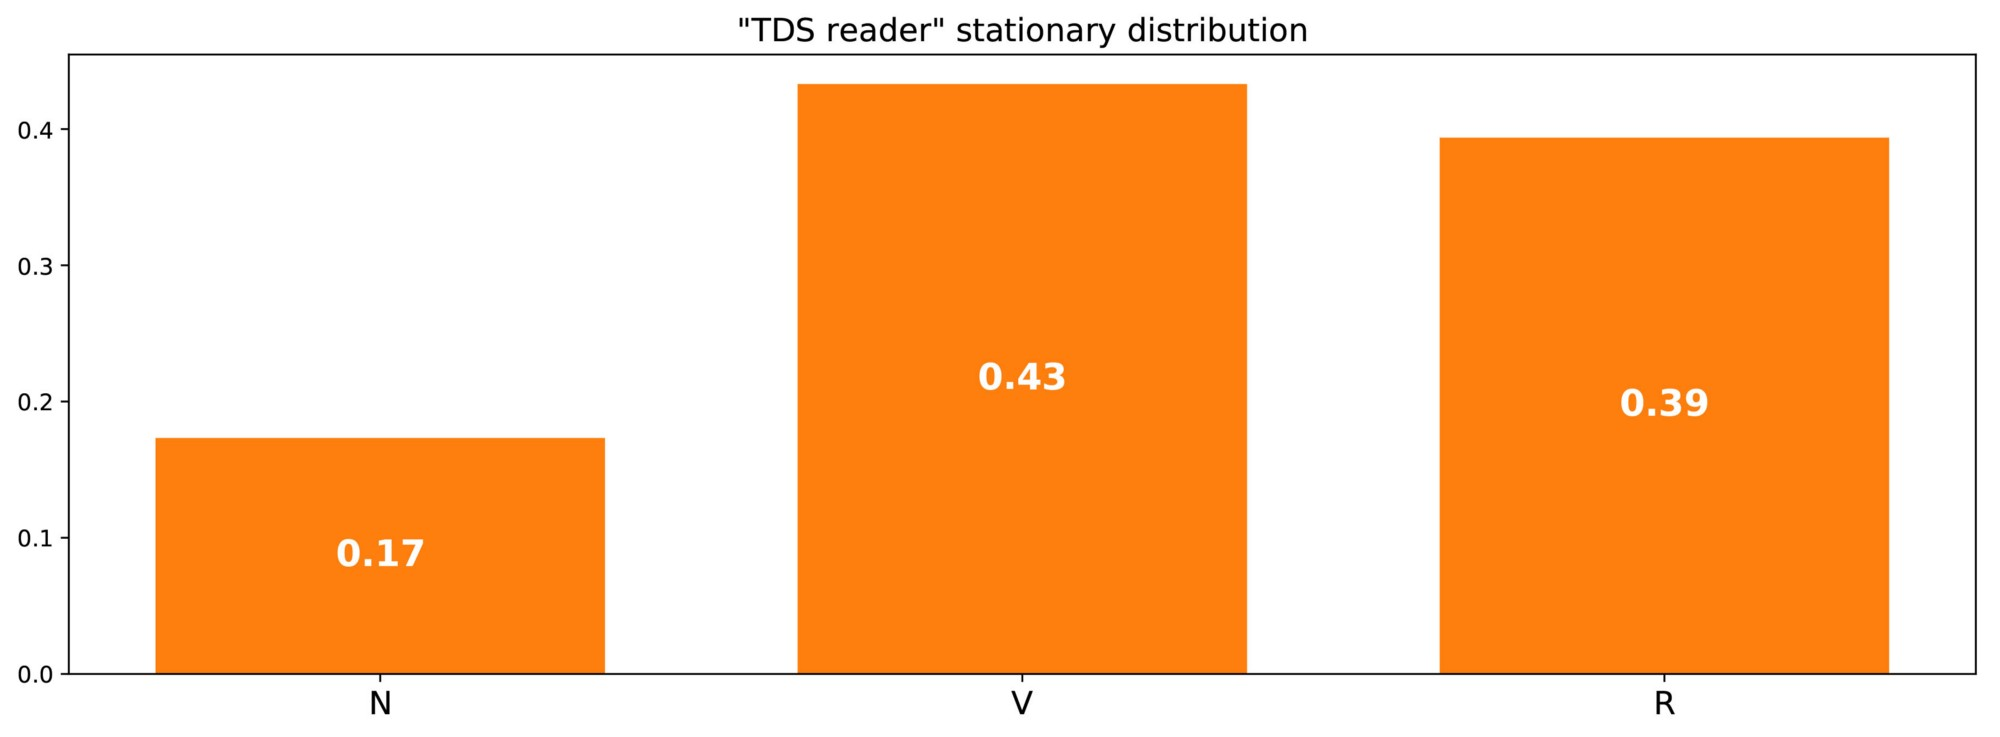
\includegraphics[width=\textwidth]{pic/p05c07-snip08.png}
    \caption{Stationary distribution of our "TDS reader" example}
    \label{fig:p05c07-snip08}
\end{figure*}


.

We can also notice the fact that $\pi(R) = 1/m(R,R)$, that is a pretty logical identity when thinking a little bit about it (but we won't give any more detail in this post).

As the chain is irreducible and aperiodic, it means that, in the long run, the probability distribution will converge to the stationary distribution (for any initialisation). Stated in another way, no matter what the initial state of our TDS reader is, if we wait long enough and pick a day randomly then we have a probability $\pi(N)$ that the reader doesn't visit for this day, a probability $\pi(V)$ that the reader visits but doesn't read and a probability $\pi(R)$ that the reader visits and reads. To better grasp that convergence property, let's take a look at the following graphic that shows the evolution of probability distributions beginning at different starting point and the (quick) convergence to the stationary distribution.


\begin{figure*}[h]
    \centering
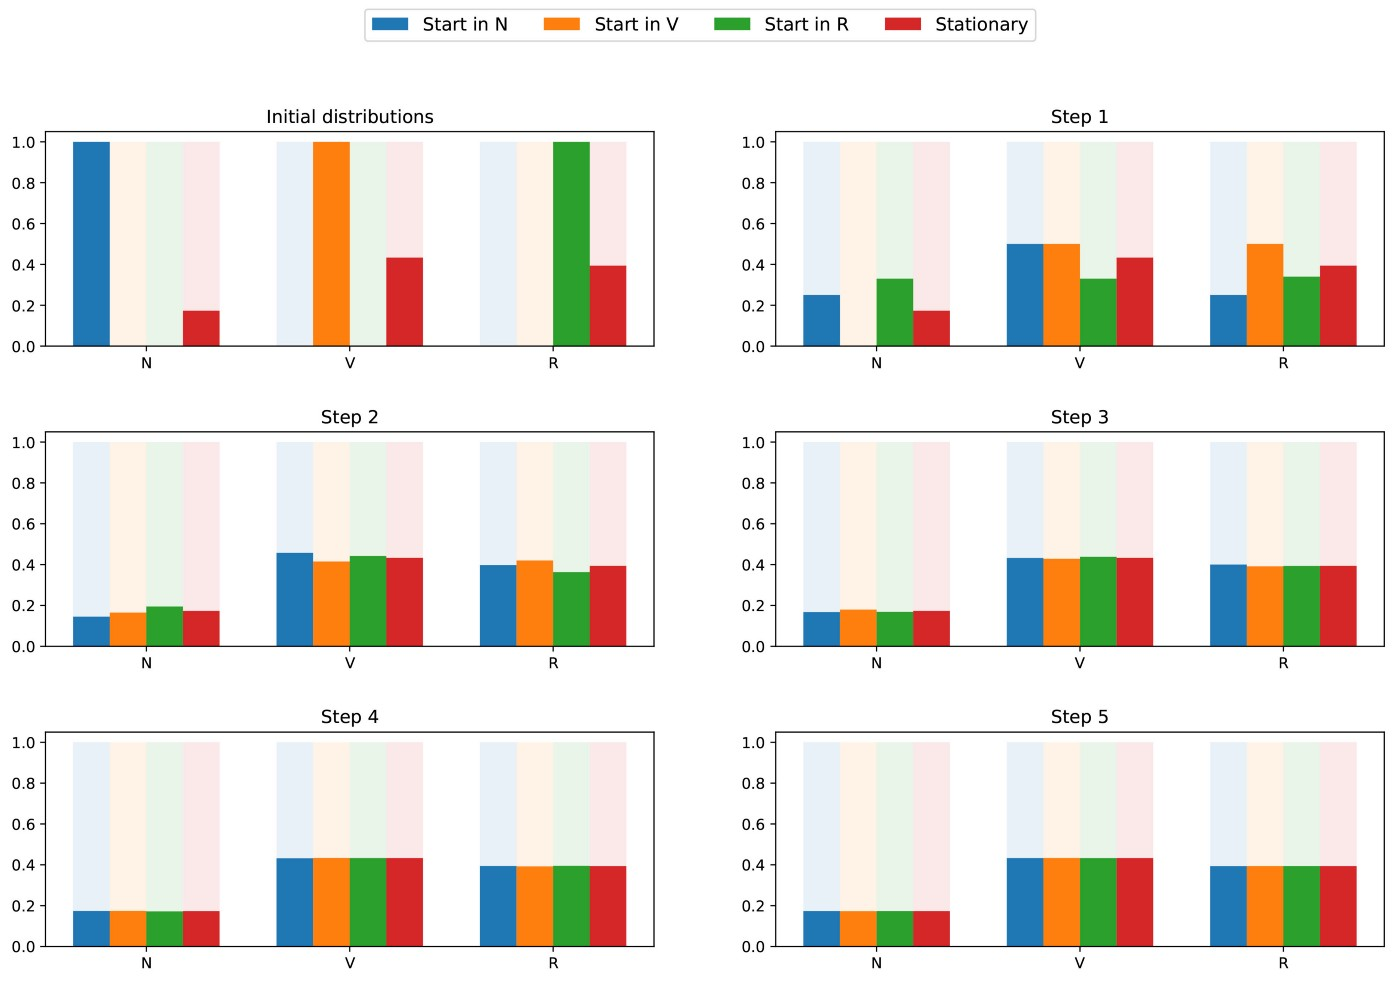
\includegraphics[width=\textwidth]{pic/p05c07-snip09.png}
    \caption[Visualisation of convergence of probability distributions]{Visualisation of the convergence of 3 differently initialised probability distributions (blue, orange and green) towards the stationary distribution (red)}
    \label{fig:p05c07-snip09}
\end{figure*}




\section{A classical example: the PageRank algorithm}

It's now time to come back to PageRank! Before going any further, let's mention the fact that the interpretation that we are going to give for the PageRank is not the only one possible and that authors of the original paper had not necessarily in mind Markov chains when designing the method. However, the following interpretation has the big advantage to be very well understandable.

\subsection{The random web surfer}

The problem PageRank tries to solve is the following: how can we rank pages of a given a set (we can assume that this set has already been filtered, for example on some query) by using the existing links between them?

To solve this problem and be able to rank the pages, PageRank proceed roughly as follows. We consider that a random web surfer is on one of the pages at initial time. Then, this surfer starts to navigate randomly by clicking, for each page, on one of the links that lead to another page of the considered set (assume that links to pages out of this set are disallowed). For a given page, all the allowed links have then equal chance to be clicked.

We have here a the setting of a Markov chain: pages are the different possible states, transition probabilities are defined by the links from page to page (weighted such that on each page all the linked pages have equal chances to be chosen) and the memoryless properties is clearly verified by the behaviour of the surfer. If we assume also that the defined chain is recurrent positive and aperiodic (some minor tricks are used to ensure we meet this setting), then after a long time the "current page" probability distribution converges to the stationary distribution. So, no matter the starting page, after a long time each page has a probability (almost fixed) to be the current page if we pick a random time step.

The hypothesis behind PageRank is that the most probable pages in the stationary distribution must also be the most important (we visit these pages often because they receive links from pages that are also visited a lot in the process). The stationary probability distribution defines then for each state the value of the PageRank.

\subsection{A toy example}

In order to make all this much clearer, let's consider a toy example. Assume that we have a tiny website with 7 pages labeled from 1 to 7 and with links between the pages as represented in the graph in Figure~\ref{fig:p05c07-snip10}.


\begin{figure*}[h]
    \centering
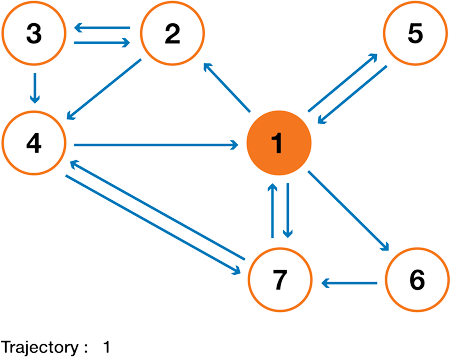
\includegraphics[width=.3\textwidth]{pic/p05c07-snip10-00.png}
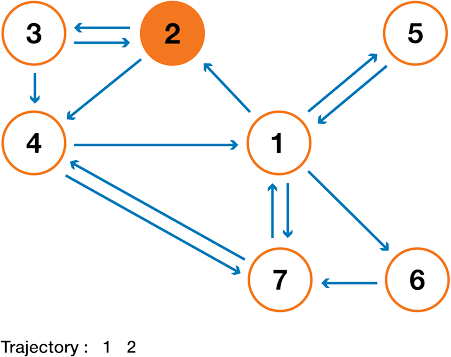
\includegraphics[width=.3\textwidth]{pic/p05c07-snip10-01.png}
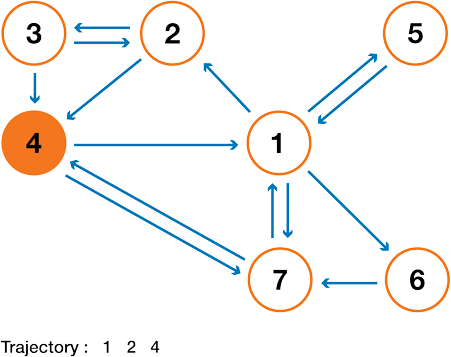
\includegraphics[width=.3\textwidth]{pic/p05c07-snip10-02.png}\\\ \\
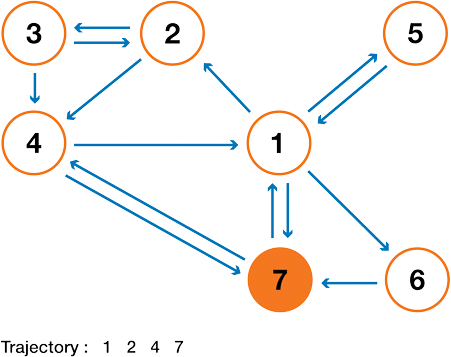
\includegraphics[width=.3\textwidth]{pic/p05c07-snip10-03.png}
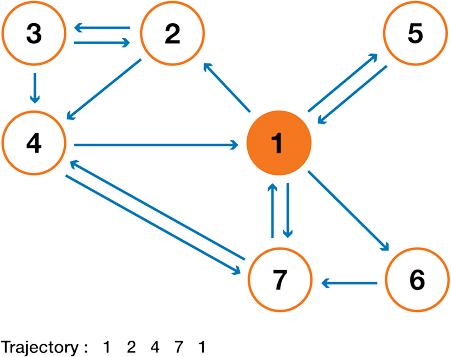
\includegraphics[width=.3\textwidth]{pic/p05c07-snip10-04.png}
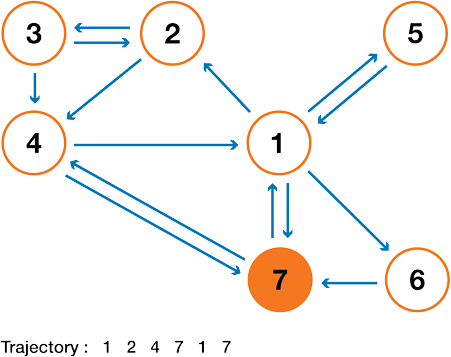
\includegraphics[width=.3\textwidth]{pic/p05c07-snip10-05.png}\\\ \\
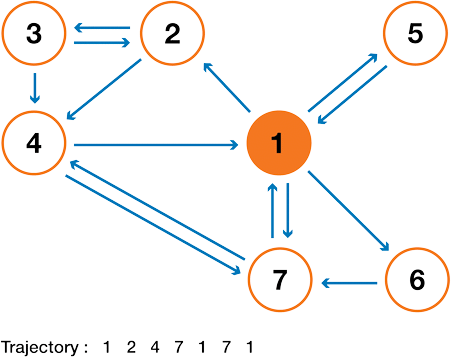
\includegraphics[width=.3\textwidth]{pic/p05c07-snip10-06.png}
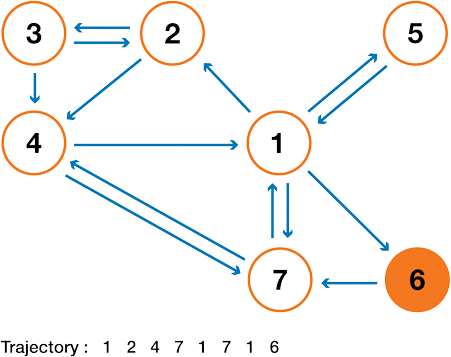
\includegraphics[width=.3\textwidth]{pic/p05c07-snip10-07.png}
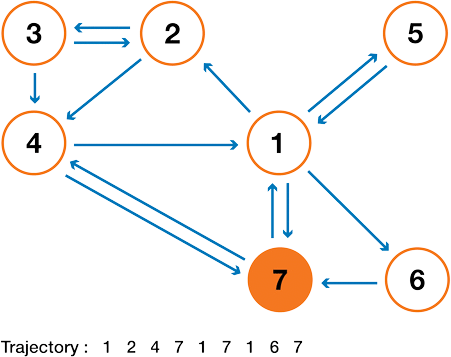
\includegraphics[width=.3\textwidth]{pic/p05c07-snip10-08.png}\\\ \\
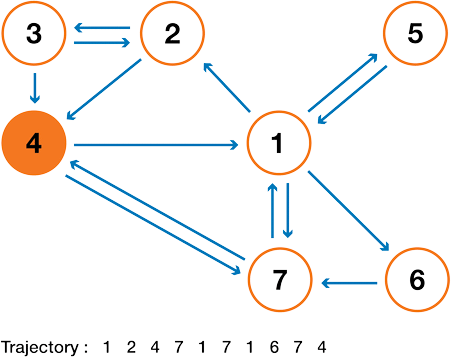
\includegraphics[width=.3\textwidth]{pic/p05c07-snip10-09.png}
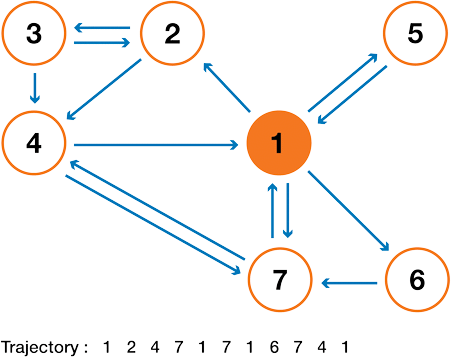
\includegraphics[width=.3\textwidth]{pic/p05c07-snip10-10.png}
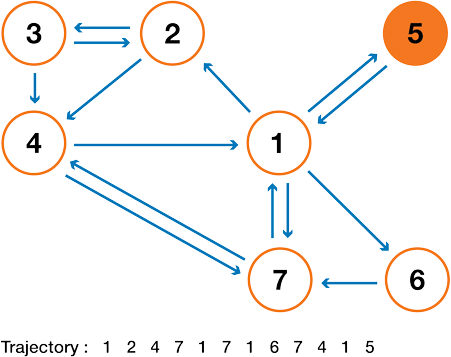
\includegraphics[width=.3\textwidth]{pic/p05c07-snip10-11.png}\\\ \\
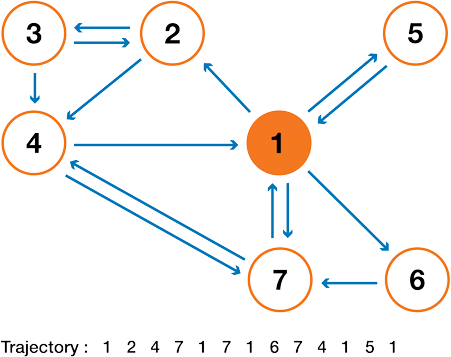
\includegraphics[width=.3\textwidth]{pic/p05c07-snip10-12.png}
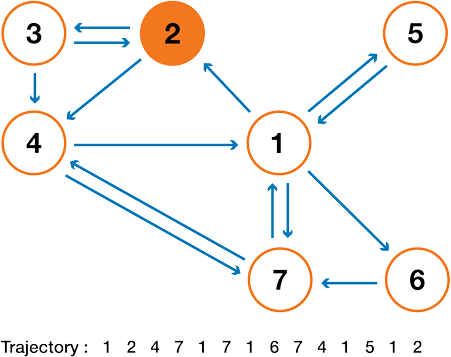
\includegraphics[width=.3\textwidth]{pic/p05c07-snip10-13.png}
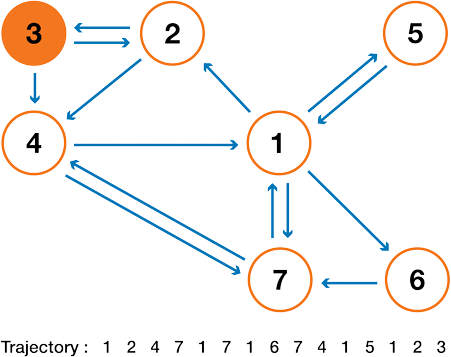
\includegraphics[width=.3\textwidth]{pic/p05c07-snip10-14.png}
    \caption{Markov chain trajectory}
    \label{fig:p05c07-snip10}
\end{figure*}

\FloatBarrier


For clarity the probabilities of each transition have not been displayed in the previous representation. However, as the "navigation" is supposed to be purely random (we also talk about "random walk"), the values can be easily recovered using the simple following rule: for a node with $K$ outlinks (a page with $K$ links to other pages), the probability of each outlink is equal to $1/K$. So, the probability transition matrix is given by
\begin{equation}p=\left(\begin{array}{ccccccc}
. & 0.25 & . & . & 0.25 & 0.25 & 0.25 \\
. & . & 0.5 & 0.5 & . & . & . \\
. & 0.5 & . & 0.5 & . & . & . \\
0.5 & . & . & . & . & . & 0.5 \\
1.0 & . & . & . & . & . & . \\
. & . & . & . & . & . & 1.0 \\
0.5 & . & . & 0.5 & . & . & .
\end{array}\right)\end{equation}
where 0.0 values have been replaced by '.' for readability. Before any further computation, we can notice that this Markov chain is irreducible as well as aperiodic and, so, after a long run the system converges to a stationary distribution. As we already saw, we can compute this stationary distribution by solving the following left eigenvector problem
\begin{equation}\begin{aligned}
&\pi=\pi_p\\
&\text { with } \quad \pi=\left(\begin{array}{lllllll}
\pi_{1} & \pi_{2} & \pi_{3} & \pi_{4} & \pi_{5} & \pi_{6} & \pi_{7}
\end{array}\right)
\end{aligned}\end{equation}
Doing so we obtain the following values of PageRank (values of the stationary distribution) for each page is shown in Figure~\ref{fig:p05c07-snip11}.
The PageRank ranking of this tiny web site is therefore\\
1 > 7 > 4 > 2 > 5 = 6 > 3.

\begin{figure*}[h]
    \centering
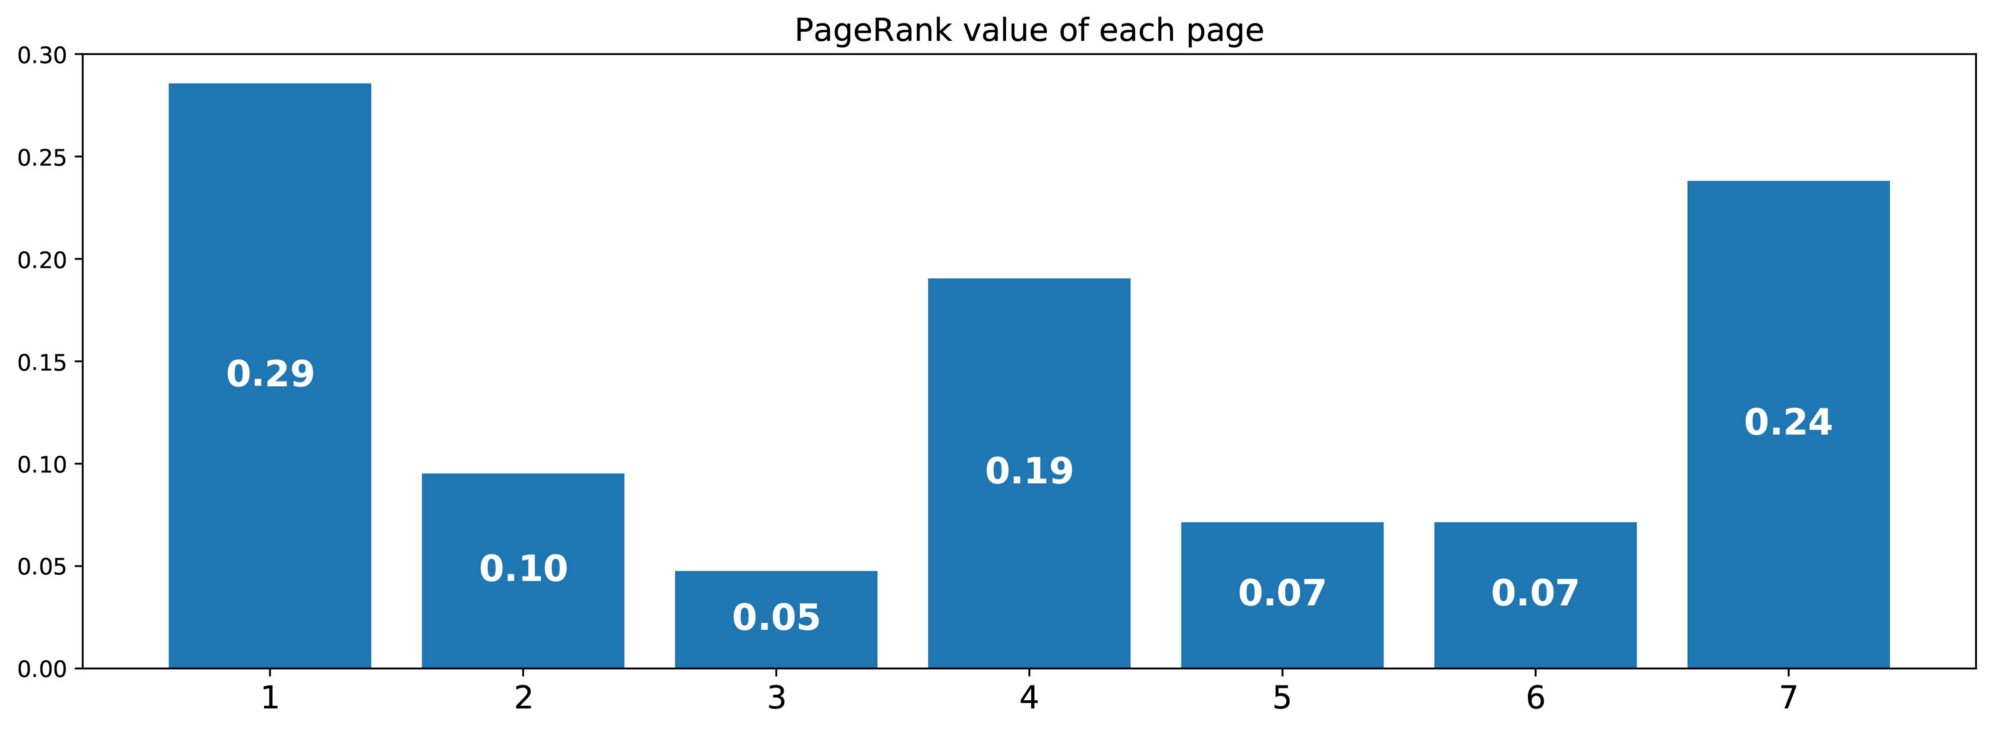
\includegraphics[width=\textwidth]{pic/p05c07-snip11.png}
    \caption{PageRank values computed on our toy example that contains 7 pages}
    \label{fig:p05c07-snip11}
\end{figure*}





\subsection{Takeaways}

The main takeaways of this article are the following:
\begin{enumerate}

\item random processes are collections of random variables, often indexed over time (indices often represent discrete or continuous time)

\item for a random process, the Markov property says that, given the present, the probability of the future is independent of the past (this property is also called "memoryless property")

\item discrete time Markov chain are random processes with discrete time indices and that verify the Markov property

\item the Markov property of Markov chains makes the study of these processes much more tractable and allows to derive some interesting explicit results (mean recurrence time, stationary distribution…)

\item one possible interpretation of the PageRank (not the only one) consists in imagining a web surfer that randomly navigates from page to page and in taking the induced stationary distribution over pages as a factor of ranking (roughly, the most visited pages in steady-state must be the one linked by other very visited pages and then must be the most relevant)
\end{enumerate}

To conclude, let's emphasise once more how powerful Markov chains are for problems modelling when dealing with random dynamics. Due to their good properties, they are used in various fields such as queueing theory \cite{willig1999} (optimising the performance of telecommunications networks, where messages must often compete for limited resources and are queued when all resources are already allocated), statistics (the well known "Markov Chain Monte Carlo" \cite{JosephRoccaBayes2019} random variables generation technique is based on Markov chains), biology (modelling of biological populations evolution), computer science (hidden Markov models \cite{Rabiner1986,Rabiner1989,stamp2018} are important tools in information theory and speech recognition) and others.

Obviously, the huge possibilities offered by Markov chains in terms of modelling as well as in terms of computation go far behind what have been presented in this modest introduction and, so, we encourage the interested reader to read more about these tools that entirely have there place in the (data) scientist toolbox.

